\newpage
\subsection{QuizziPedia::Front-End::Views}

\label{QuizziPedia::Front-End::Views}
\begin{figure}[ht]
	\centering
	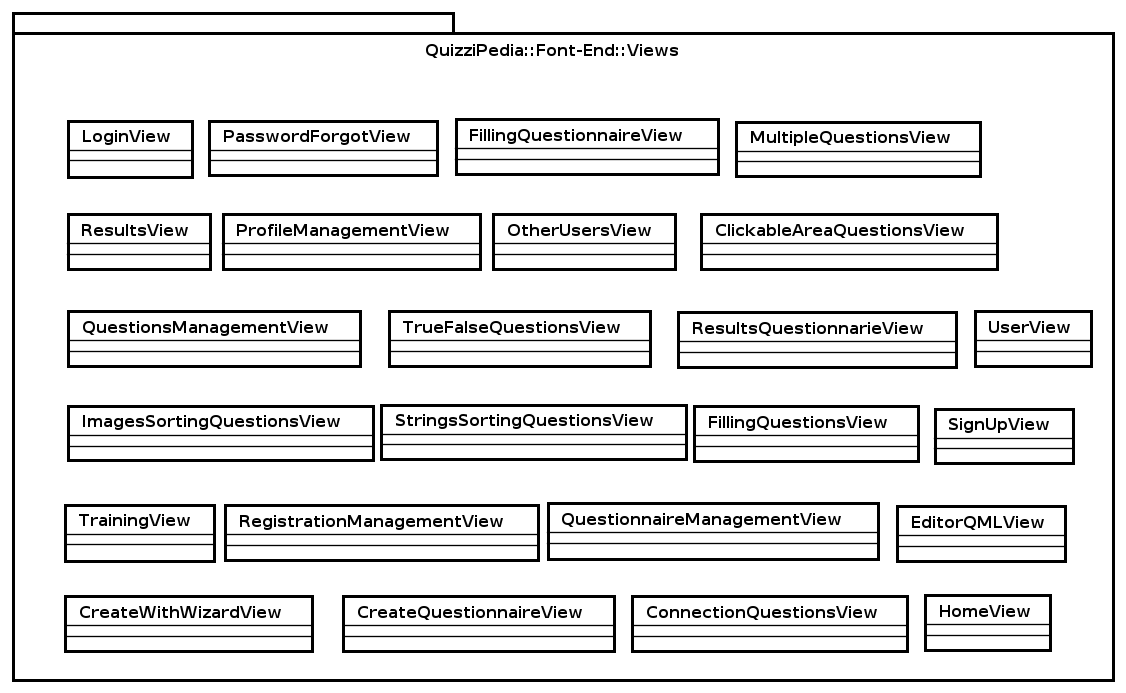
\includegraphics[scale=0.50]{UML/Package/QuizziPedia_Front-End_Views.png}
	\caption{QuizziPedia::Front-End::Views}
\end{figure}\FloatBarrier
\begin{itemize}
	\item \textbf{Descrizione}: package contenente le views front-end dell'applicazione;
	\item \textbf{Padre}: \texttt{Front-End};
	\item \textbf{Interazione con altri componenti}:
	\begin{itemize}
		\item \texttt{Controllers}: package contenente i \textit{controllers\ped{G}} Front-End dell'applicazione;
		\item \texttt{Directives}: package contenente le \textit{directives\ped{G}} Front-End dell'applicazione.
	\end{itemize}
	\item \textbf{Classi contenute}:
	\begin{itemize}
		\item \texttt{LoginView}: classe contenente le form necessarie per effettuare il login. Contiene inoltre un link alla pagina di registrazione e uno alla pagina per il recupero della password;
		\item \texttt{SignUpView}: classe contenente le form dedicate alla registrazione utente. Contiene inoltre un link alla pagina di login;
		\item \texttt{PasswordForgotView}: classe contenente le form necessarie per il recupero della password dimenticata;
		\item \texttt{HomeView}: classe contenente la direttiva per barra di ricerca degli utenti e questionari e il bottone che porterà l'utente nella modalità allenamento;
		\item \texttt{ResultsView}: classe contenente i risultati della ricerca effettuata. Vengono visualizzati sia gli utenti che i questionari trovati;
		\item \texttt{UserView}: contenente le direttive dei dati personali dell'utente, delle sue statistiche relative ai questionari e agli allenamenti effettuati e dei questionari a cui è iscritto;
		\item \texttt{OtherUserView}: classe contenente le direttive dei dati personali e delle statistiche di un utente ricercato;
		\item \texttt{ProfileManagementView}: classe contenente i dati personali che un utente può modificare dopo essersi registrato al sistema;
		\item \texttt{QuestionsManagementView}: classe contenente l'elenco delle domande create;
		\item \texttt{TrueFalseQuestionView}: classe contenente le direttive per creare una domanda vero/falso;
		\item \texttt{MultipleQuestionView}: classe contenente le direttive per creare una domanda a risposta multipla;
		\item \texttt{ConnectionQuestionView}: classe contenente i campi e le direttive per creare una domanda a collegamento;
		\item \texttt{ImagesSortingQuestionView}: classe contenente i campi e le direttive per creare una domanda a ordinamento immagini;
		\item \texttt{StringsSortingQuestionView}: classe contenente i campi e le direttive per creare una domanda a ordinamento stringhe;
		\item \texttt{FillingQuestionsView}: classe contenente i campi e le direttive per creare una domanda a riempimento testo;
		\item \texttt{ClickableAreaQustionView}: classe contenente i campi e le direttive per creare una domanda ad area cliccabile;
		\item \texttt{EditorQMLView}: classe contenente l'editor \textit{QML\ped{G}} per la creazione di domande personalizzate;
		\item \texttt{TrainingView}: classe principale della modalità allenamento; conterrà i vari templates di ogni domanda dell'allenamento;
		\item \texttt{FillingQuestionnaireView}: classe principale per la compilazione del questionario; conterrà i vari templates di ogni domanda appartenente al questionario;
		\item \texttt{QuestionnaireManagementView}: classe principale per la gestione dei questionari;
		\item \texttt{CreateQuestionnaireView}: classe per la creazione del questionario;
		\item \texttt{ResultQuestionnaireView}: classe contenente i risultati conseguiti dagli utenti che hanno compilato il proprio questionario;
		\item \texttt{RegiastrationManagementView}: classe che permette di visualizzare gli utenti iscritti ad un questionario.
	\end{itemize}
\end{itemize}